%! Author = lili
%! Date = 8/13/26

\section{Abgabe 2.4}\label{sec:abgabe-2.4}

\subsection{HA 2.4.1 \teils}\label{subsec:ha-2.4.1}
Die unten stehenden Werte sind Druckfestigkeiten (in $0.1\,$N/mm$^2$), welche an 30 Betonwürfeln ermittelt wurden:
\begin{center}
    \begin{tabular}{cccccccccc}
        374 & 358 & 341 & 355 & 342 & 334 & 353 & 346 & 355 & 344 \\
        349 & 330 & 352 & 328 & 336 & 359 & 361 & 345 & 324 & 386 \\
        335 & 371 & 358 & 328 & 353 & 352 & 366 & 354 & 378 & 324 \\
    \end{tabular}
\end{center}
(aus: H.\ Riedwyl: \emph{Angewandte mathematische Statistik in Wissenschaft, Administration und Technik}, 1978)

\begin{auf}[(a) Fertigen Sie ein geeignetes Histogramm zu diesen Daten an.]
    $\ $
    \begin{figure}[H]
        \centering
        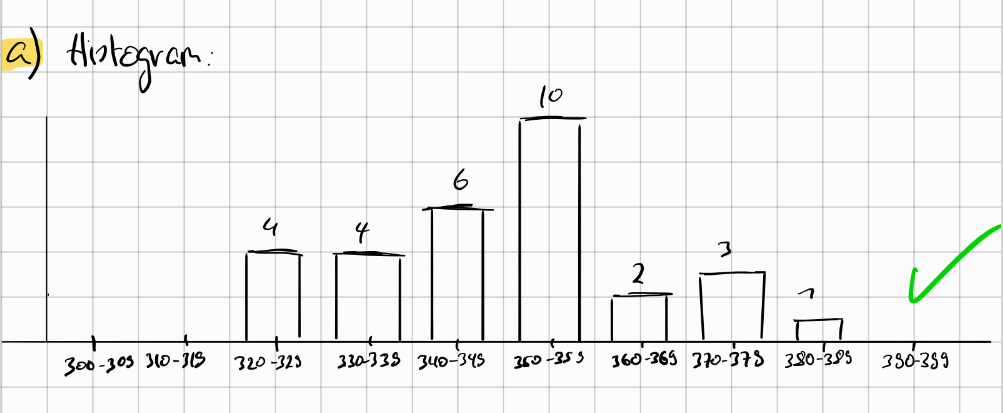
\includegraphics[width=0.8\linewidth]{images/lösungen/wts241a}\label{fig:figure68}
    \end{figure}
\end{auf}

\begin{auf}[(b) Bestimmen Sie arithmetisches Mittel, Median und Modalwert der Stichprobe.]
    $\ $
    \begin{figure}[H]
        \centering
        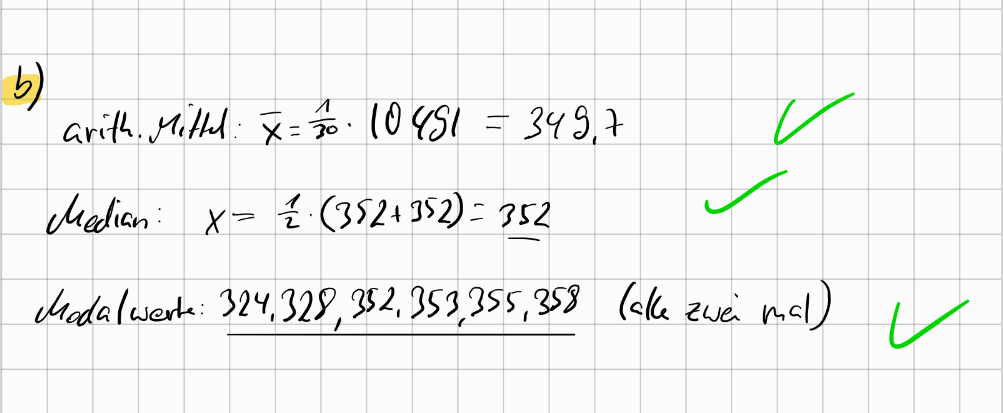
\includegraphics[width=0.8\linewidth]{images/lösungen/wts241b}\label{fig:figure67}
    \end{figure}
\end{auf}

\begin{auf}[(c) Bestimmen Sie das untere Quartil und das 90\%-Quantil der Stichprobe.]
    $\ $
    \begin{figure}[H]
        \centering
        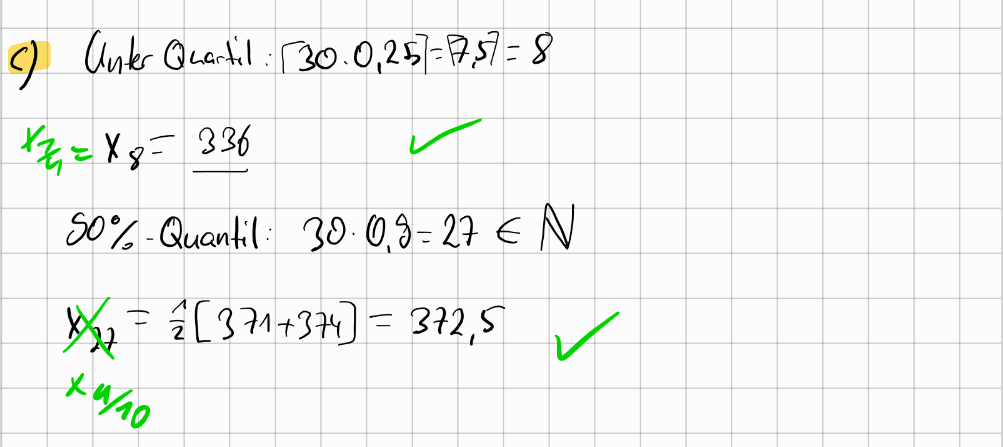
\includegraphics[width=0.8\linewidth]{images/lösungen/wts241c}\label{fig:figure66}
    \end{figure}
\end{auf}

\begin{auf}[(d) Bestimmen Sie die Spannweite, den Quartilsabstand, den 10\%-Quantilsabstand und die Medianabweichung der Stichprobe.]
    $\ $
    \begin{figure}[H]
        \centering
        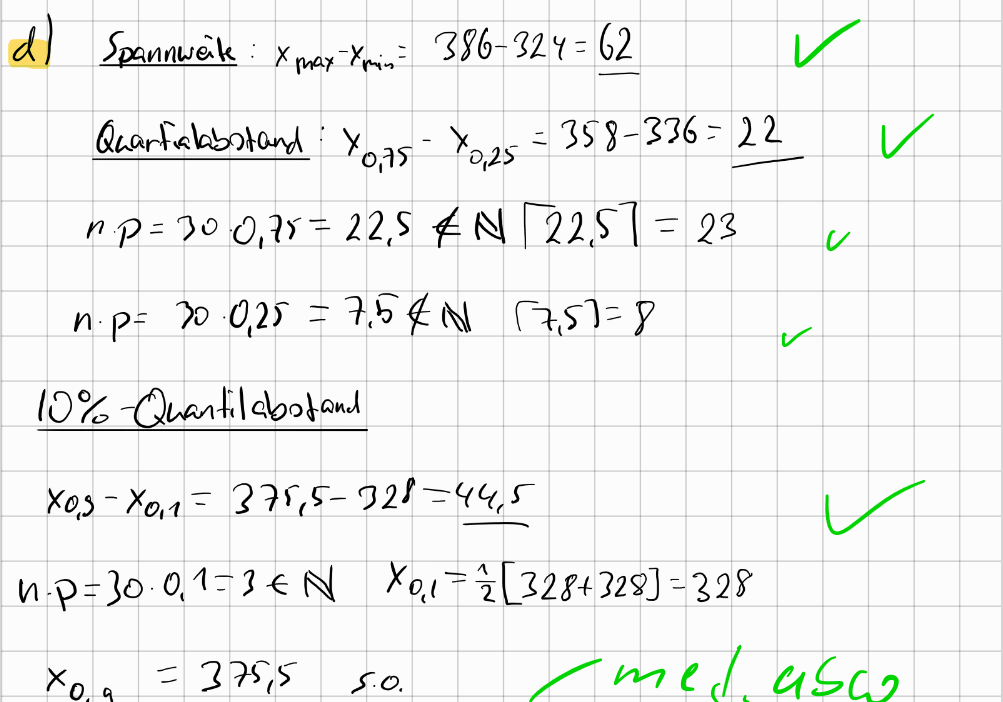
\includegraphics[width=0.8\linewidth]{images/lösungen/wts241d}\label{fig:figure65}
    \end{figure}
\end{auf}

\begin{auf}[(e) Bestimmen Sie die mittlere absolute Abweichung vom Median und vom arithmetischen Mittel.]
    $\ $
    \begin{figure}[H]
        \centering
        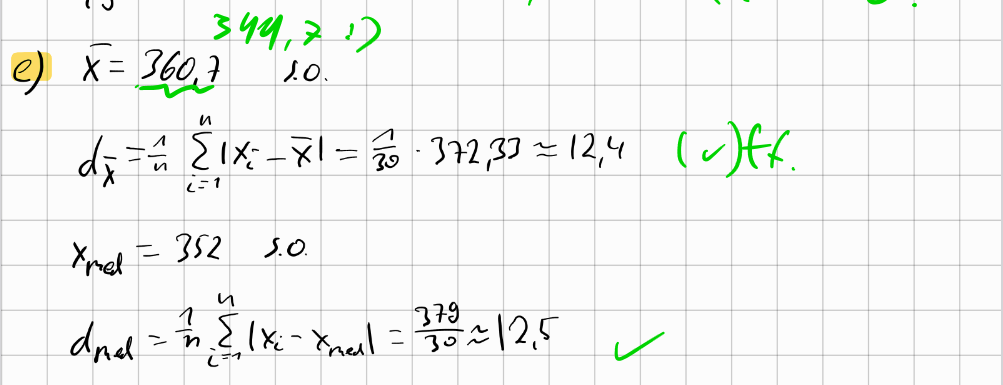
\includegraphics[width=0.8\linewidth]{images/lösungen/wts241e}\label{fig:figure64}
    \end{figure}
\end{auf}

\begin{auf}[(f)  Bestimmen Sie die Varianz und Standardabweichung der Stichprobe.]
    $\ $
    \begin{figure}[H]
        \centering
        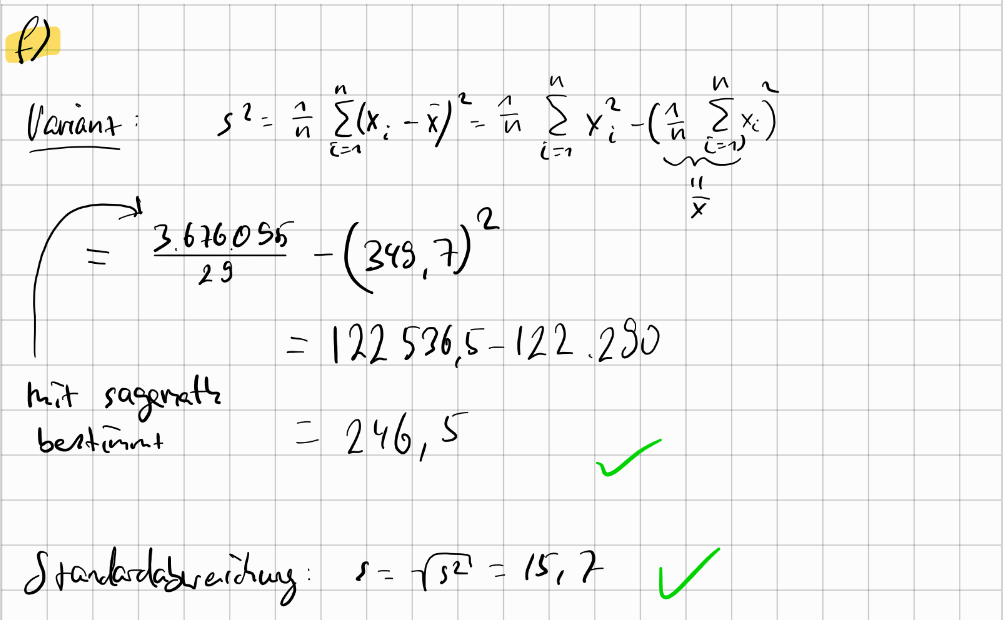
\includegraphics[width=0.8\linewidth]{images/lösungen/wts241f}\label{fig:figure63}
    \end{figure}
\end{auf}

\begin{auf}[(g) Wie groß kann der Median der oben genannten Daten höchstens werden, wenn beliebige 4 der 30 Werte verzehnfacht werden? Begründen Sie Ihre Antwort.]
    NOCH KEINE LÖSUNG % TODO NOCH KEINE LÖSUNG
\end{auf}

\subsection{HA 2.4.2 \abhaken}\label{subsec:ha-2.4.2}

Zeigen Sie, dass die folgenden Sachen Lagemaße sind:

\begin{auf}[(a) Spannweite]
    $\ $
    \begin{figure}[H]
        \centering
        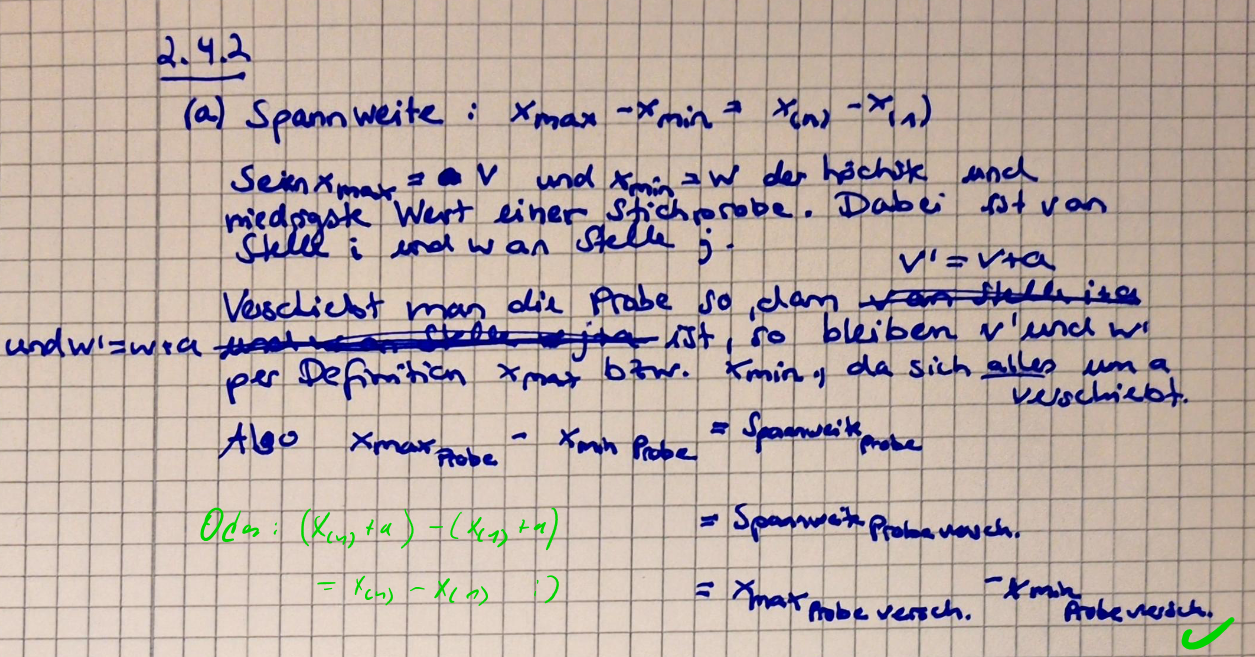
\includegraphics[width=0.8\linewidth]{images/lösungen/wts242a}\label{fig:figure62}
    \end{figure}
\end{auf}

\begin{auf}[(b) Quartilsabstand]
    $\ $
    \begin{figure}[H]
        \centering
        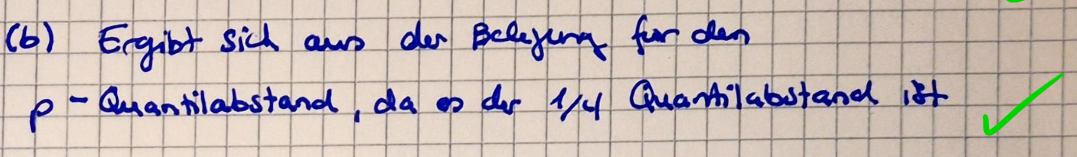
\includegraphics[width=0.8\linewidth]{images/lösungen/wts242b}\label{fig:figure61}
    \end{figure}
\end{auf}

\begin{auf}[(c) $p$-Quantilsabstand]
    $\ $
    \begin{figure}[H]
        \centering
        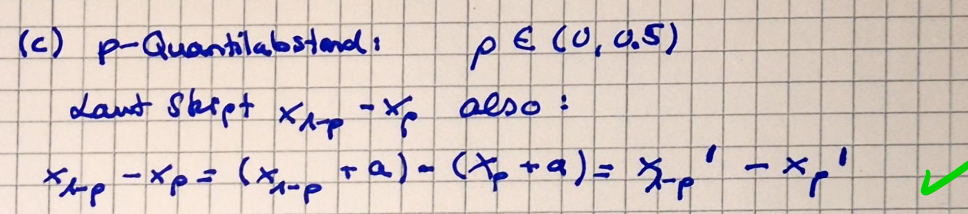
\includegraphics[width=0.8\linewidth]{images/lösungen/wts242c}\label{fig:figure60}
    \end{figure}
\end{auf}

\begin{auf}[(d) Medianabweichung]
    $\ $
    \begin{figure}[H]
        \centering
        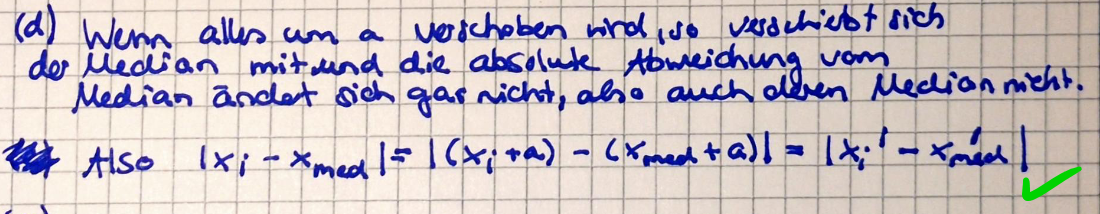
\includegraphics[width=0.8\linewidth]{images/lösungen/wts242d}\label{fig:figure59}
    \end{figure}
\end{auf}

\begin{auf}[(e)  mittlere absolute Abweichung vom Median]
    $\ $
    \begin{figure}[H]
        \centering
        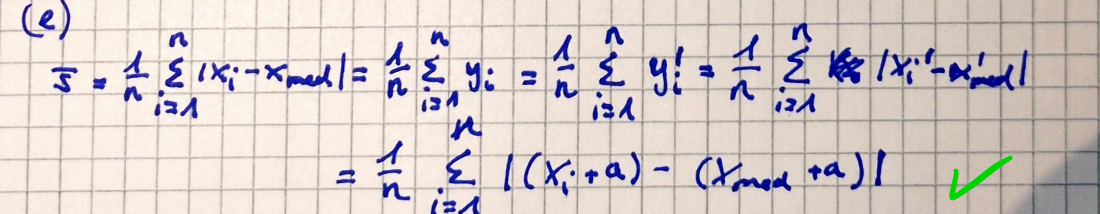
\includegraphics[width=0.8\linewidth]{images/lösungen/wts242e}\label{fig:figure58}
    \end{figure}
\end{auf}

\begin{auf}[(f) mittlere absolute Abweichung vom arithmetischen Mittel]
    $\ $
    \begin{figure}[H]
        \centering
        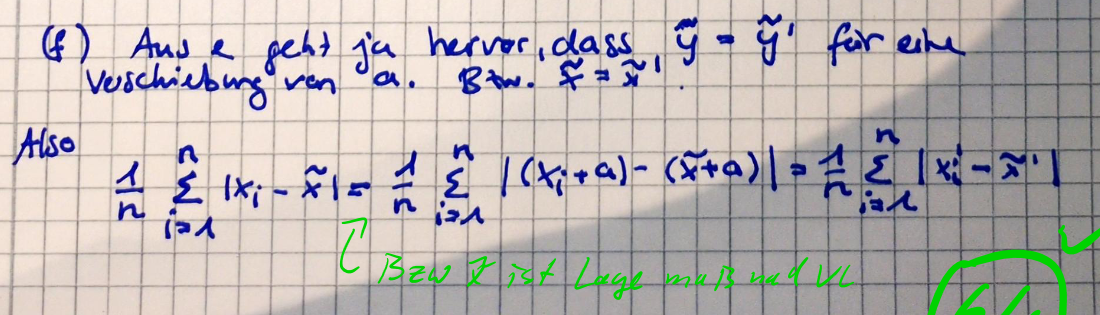
\includegraphics[width=0.8\linewidth]{images/lösungen/wts242f}\label{fig:figure57}
    \end{figure}
\end{auf}

\subsection{HA 2.4.3 \teils}\label{subsec:ha-2.4.3}
Wir betrachten ein zweimal unabhängig durchgeführtes Bernoulli-Experiment mit unbekannter Erfolgswahrscheinlichkeit $\theta\in(0,1)$.
Sie können sich das zweimalige Werfen einer Reißzwecke vorstellen.
\textit{In dieser Aufgabe vergleichen Sie arithmetisches und geometrisches Mittel als Schätzer.}

\begin{auf}[(a) Geben Sie das zugehörige statistische Modell vollständig an. Welche Angaben müssen Sie dafür machen?]
    NOCH KEINE LÖSUNG % TODO NOCH KEINE LÖSUNG
\end{auf}

\begin{auf}[(b) Aus der Vorlesung wissen wir, dass $t_1$, gegeben durch $t_1(x)=\frac12(x_1+x_2)$ für alle $x\in\mathcal X$, ein erwartungstreuer Schätzer für $\theta$ ist mit Risiko $R(\theta,t_1)=\frac12\theta(1-\theta)$ für alle $\theta\in\Theta$. Geben Sie Verweise auf die entsprechenden Resultate der Vorlesung.]
    NOCH KEINE LÖSUNG % TODO NOCH KEINE LÖSUNG
\end{auf}

\begin{auf}[(c) Begründen Sie, warum auch $t_2$ mit $t_2(x)=\sqrt{x_1\cdot x_2}$ für alle $x\in\mathcal X$ ein Schätzer für $\theta$ ist.]
    $\ $
    \begin{figure}[H]
        \centering
        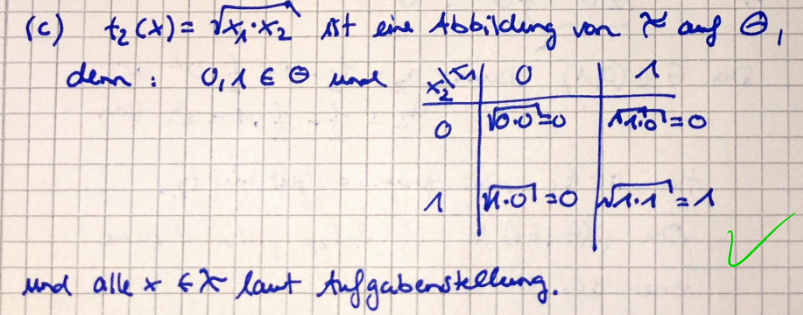
\includegraphics[width=0.8\linewidth]{images/lösungen/wts243c}\label{fig:figure56}
    \end{figure}
\end{auf}
Beachten Sie, dass im Kontext der Aufgabe $\sqrt{x_1\cdot x_2}=x_1\cdot x_2=(x_1\cdot x_2)^2$ genutzt werden kann, da nur $x_1,x_2\in\{0,1\}$ auftreten.
Dies vereinfacht die Berechnungen.
\begin{auf}[(d) Berechnen Sie Bias und Risiko von $t_2$.]
    NOCH KEINE LÖSUNG % TODO NOCH KEINE LÖSUNG
\end{auf}

\begin{auf}[(e) Ist $t_1$ mindestens so gut wie $t_2$? Ist einer der beiden Schätzer besser als der andere?]
    NOCH KEINE LÖSUNG % TODO NOCH KEINE LÖSUNG
\end{auf}
